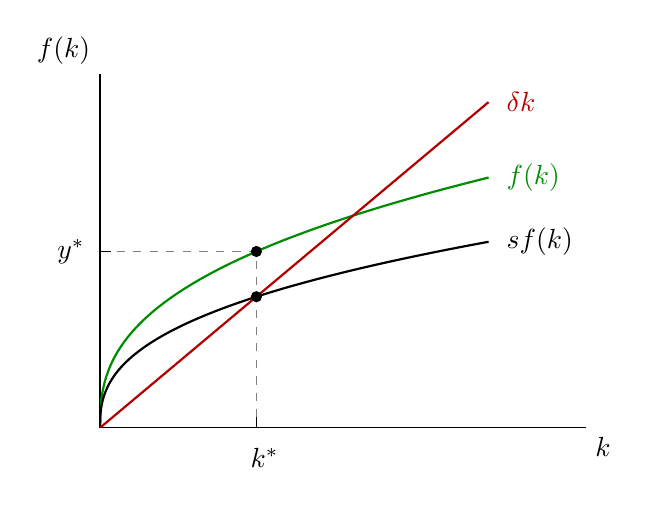
\begin{tikzpicture}[x=1bp,y=1bp]
  % Parameters (no custom commands)
  \pgfmathsetmacro{\alpha}{0.385}
  \pgfmathsetmacro{\A}{1.0}
  \pgfmathsetmacro{\kstarTarget}{56.29872}
  \pgfmathsetmacro{\ystarTarget}{63.4818}
  \pgfmathsetmacro{\ysfTarget}{47.189}
  \pgfmathsetmacro{\s}{\ysfTarget/\ystarTarget}
  \pgfmathsetmacro{\deltaParam}{\ysfTarget/\kstarTarget}

  % Derived steady state and scales
  \pgfmathsetmacro{\kstar}{pow(\s*\A/\deltaParam, 1/(1-\alpha))}
  \pgfmathsetmacro{\ystar}{\A*pow(\kstar,\alpha)}
  \pgfmathsetmacro{\ysf}{\s*\ystar}
  \pgfmathsetmacro{\xscale}{\kstarTarget/\kstar}
  \pgfmathsetmacro{\yscale}{\ystarTarget/\ystar}

  % Pixel-space values
  \pgfmathsetmacro{\kstarPix}{\kstar*\xscale}
  \pgfmathsetmacro{\ystarPix}{\ystar*\yscale}
  \pgfmathsetmacro{\ysfPix}{\ysf*\yscale}

  % Geometry and extents (numerical values inlined)
  \pgfmathsetmacro{\AxisEndX}{0.90*194.27399}
  \pgfmathsetmacro{\curveEnd}{0.80*\AxisEndX}
  \pgfmathsetmacro{\deltaEnd}{\deltaParam*(\curveEnd)}
  \pgfmathsetmacro{\AxisEndY}{\deltaEnd + 10}

  \begin{axis}[
      scale only axis,
      width=194.27399bp,
      height=161.39407bp,
      at={(10bp,10bp)},
      anchor=south west,
      xmin=0, xmax=194.27399,
      ymin=0, ymax=161.39407,
      axis lines=none,
      tick style={draw=none},
      xtick=\empty, ytick=\empty,
      clip mode=individual,
    ]

    % Axes (shortened)
    \draw[line width=0.3985pt, line cap=butt]
      (axis cs:0,0) -- (axis cs:\AxisEndX,0);
    \draw[line width=0.3985pt, line cap=butt]
      (axis cs:0,0) -- (axis cs:0,\AxisEndY);

    % f(k): green concave curve
    \addplot [domain=0:\curveEnd, samples=900, no marks, line width=0.79701pt,
               color={rgb,1:red,0;green,0.55;blue,0}]
      ({x}, {\yscale*\A*pow(x/\xscale,\alpha)});

    % s f(k): black curve
    \addplot [domain=0:\curveEnd, samples=900, no marks, line width=0.79701pt, color=black]
      ({x}, {\yscale*\s*\A*pow(x/\xscale,\alpha)});

    % \delta k line (brown-red)
    \addplot [domain=0:\curveEnd, samples=2, no marks, line width=0.79701pt,
               color={rgb,1:red,0.7;green,0;blue,0}]
      ({x}, {\deltaParam*(x)});

    % Dashed guides at steady state (k*, y*)
    \draw[line width=0.3985pt, line cap=butt, line join=miter,
          dash pattern=on 2.98883pt off 2.98883pt, color=gray]
      (axis cs:0,\ystarPix) -- (axis cs:\kstarPix,\ystarPix) -- (axis cs:\kstarPix,0);

    % Tick marks (all inside: above x-axis, to the right of y-axis)
    \draw[line width=0.3985pt] (axis cs:\kstarPix,0) -- (axis cs:\kstarPix,4);
    \draw[line width=0.3985pt] (axis cs:0,\ystarPix) -- (axis cs:4,\ystarPix);

    % Dots
    \pgfmathsetmacro{\dotRadius}{1.8pt}
    \draw[line width=0.3985pt, fill=black] (axis cs:\kstarPix,\ystarPix) circle[radius=\dotRadius];
    \draw[line width=0.3985pt, fill=black] (axis cs:\kstarPix,\ysfPix) circle[radius=\dotRadius];

    % Label positions at curve end
    \pgfmathsetmacro{\fEnd}{\yscale*\A*pow(\curveEnd/\xscale,\alpha)}
    \pgfmathsetmacro{\sfEnd}{\yscale*\s*\A*pow(\curveEnd/\xscale,\alpha)}
    \pgfmathsetmacro{\deltaEnd}{\deltaParam*(\curveEnd)}

    % Curve labels
    \node[anchor=west, color={rgb,1:red,0;green,0.55;blue,0}] at (axis cs:\curveEnd+3,\fEnd) {\(f(k)\)};
    \node[anchor=west, color=black] at (axis cs:\curveEnd+3,\sfEnd) {\(sf(k)\)};
    \node[anchor=west, color={rgb,1:red,0.7;green,0;blue,0}] at (axis cs:\curveEnd+3,\deltaEnd) {\(\delta k\)};

    % Axis tick labels
    \node[anchor=north, xshift=0.3em] at (axis cs:\kstarPix,-4) {\(k^{*}\)};
    \node[anchor=east, xshift=-2pt] at (axis cs:0,\ystarPix) {\(y^{*}\)};

    % Axis titles
    \node[anchor=north west] at (axis cs:\AxisEndX,0) {\(k\)};
    \node[anchor=south east] at (axis cs:0,\AxisEndY) {\(f(k)\)};

  \end{axis}
\end{tikzpicture}
